\documentclass[11pt]{article}
\usepackage[utf8]{inputenc}
\usepackage{amsmath, amssymb, amsthm}
\usepackage{geometry}
\usepackage{algorithm}
\usepackage{algpseudocode}
\usepackage{tikz}
\geometry{a4paper, margin=1in}

\title{Mastery Test 2 - Algorithms and Complexity}
\author{Lucas Frykman}
\date{}

\begin{document}
\maketitle
\section{Problem 1}

Lets refer to the $n$ intersections and $m$ as the vertices and edges of a undirected graph $G=(V,E)$. 
where $V = \{v_i : i\in(1...n)\}$ defining each vertex's state as a portal and and 
$E = \{(e_i) =(\{u_i,v_i\},t_i): i\in{1..m}\} $ being a set of weighted edges. My approach will be to reduce this optimization problem in to problem
Dijkstra's algorithm can solve. Lets redefine each portal vertex 
(illustrated as a circle inscribing a square where the square is 
underworld and the circle is overworld) 
as sharing an edge and infact lets have every vertex in $G$ be split in to overworld and underworld pairs of vertices. 

 
\begin{figure}
    \centering
    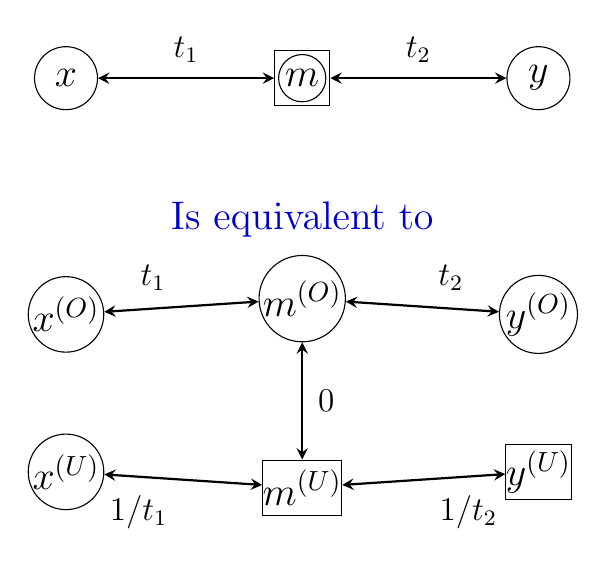
\begin{tikzpicture}[
        circ/.style={circle, draw, minimum size=0.8cm, inner sep=0pt, font=\Large},
        rect/.style={rectangle, draw, minimum size=0.7cm, inner sep=0pt, font=\Large},
        >=stealth
    ]

    % Top graph
    \node[circ] (x1) at (0,0) {$x$};
    % User's specific modification: empty square with a circle drawn inside
    \node[rect, inner sep=0pt] (mid1) at (3,0) {$m$};
    \draw (mid1.center) circle (0.3cm); % Adjust radius to fit cleanly inside
    \node[circ] (y1) at (6,0) {$y$};

    \draw[<->, thick] (x1) -- node[above=2pt, font=\large] {$t_1$} (mid1);
    \draw[<->, thick] (mid1) -- node[above=2pt, font=\large] {$t_2$} (y1);

    % Text
    \node[font=\Large, text=blue!80!black] at (3,-1.8) {Is equivalent to};

    % Bottom graph (unchanged)
    \node[circ] (x2_o) at (0,-3) {$x^{(O)}$};
    \node[circ] (x2_u) at (0,-5) {$x^{(U)}$};
    \node[circ] (mid_o) at (3,-2.8) {$m^{(O)}$};
    \node[rect] (mid_n) at (3,-5.2) {$m^{(U)}$};
    \node[circ] (y2_o) at (6,-3) {$y^{(O)}$};
    \node[rect] (y2_u) at (6,-5) {$y^{(U)}$};

    \draw[<->, thick] (x2_o) -- node[above left=2pt, font=\large] {$t_1$} (mid_o);
    \draw[<->, thick] (mid_o) -- node[above right=2pt, font=\large] {$t_2$} (y2_o);
    \draw[<->, thick] (x2_u) -- node[below left=2pt, font=\large] {$1/t_1$} (mid_n);
    \draw[<->, thick] (mid_n) -- node[below right=2pt, font=\large] {$1/t_2$} (y2_u);
    \draw[<->, thick] (mid_o) -- node[right=2pt, font=\large] {$0$} (mid_n);

    \end{tikzpicture}
    \caption{Mapping the information of the first graph to a new graph to handle portal edges}
\end{figure}

% \begin{algorithm}
% \caption{Graph to Graph remapping then solve with Dijkstra's algorithm}
% \begin{algorithmic}[1]
% \Require Weight matrix $A \in \mathbb{R}^{n\times n}$ with elements representing non-connected vertices set to $\infty$, boolean portal vector $P \in \mathbb{Z}_2^n$, integers $x, y \in \{1..n\}$

% \State $k \gets \sum_{i=1}^n p_i$ \Comment{Count the number of portals}
% % \State $N \gets n+k$
% \State $c \gets 1$
% \State Construct weight matrix $B \in \mathbb{R}^{n+k\times n+k}$ with each element initialized to $\infty$

% \For{$i = 1$ to $n$}
%     \If{$p[i] = 1$}
%         \State $B[i, n+c] \gets 0$ \Comment{nether to overworld portal edge}
%         \State $B[n+c, i] \gets 0$ \Comment{Overworld to nether to portal edge}
%         \For{$j = 1$ to $n$}
%             \State $B[i, j] \gets A[i, j]$ \Comment{Copy original weights for portal vertices}
%             \If{$j\neq x$, $j\neq y$}
%                 \State $B[n+c, j] \gets 1/A[i, j]$
%             \EndIf
%         \EndFor
%         \State $c \gets c + 1$ \Comment{Move to the next overworld vertex}
%     \Else
%         \For{$j = 1$ to $n$}
%             \State $B[i, j] \gets A[i, j]$ \Comment{Copy original weights for non-portal vertices}
%         \EndFor
%     \EndIf
% \EndFor

% \State \Comment{Execute adjacency-matrix Dijkstra's algorithm}
% \State $D \gets$ array of size $n+k$ initialized to $\infty$
% \State $\textit{Q}_{visited} \gets$ array of size $n+k$ initialized to $\textbf{false}$
% \State $D[x] \gets 0$

% \For{$t = 1$ to $n+k$}
%     \State $u \gets \textsc{Nil}$
%     \State $\textit{best} \gets \infty$

%     \For{$v = 1$ to $n+k$}
%         \If{$\textit{Q}_{visited}[v] = \textbf{false}$ \textbf{and} $D[v] < \textit{best}$}
%             \State $\textit{best} \gets D[v]$
%             \State $u \gets v$
%         \EndIf
%     \EndFor

%     \If{$u = \textsc{Nil}$}
%         \State \textbf{break}
%     \EndIf

%     \If{$u = y$}
%         \State \Return $D[y]$ \Comment{Shortest path found}
%     \EndIf

%     \State $\textit{Q}_{visited}[u] \gets \textbf{true}$

%     \For{$v = 1$ to $n+k$}
%         \If{$\textit{Q}_{visited}[v] = \textbf{false}$ \textbf{and} $B[u, v] \neq \infty$}
%             \If{$D[u] + B[u, v] < D[v]$}
%                 \State $D[v] \gets D[u] + B[u, v]$
%             \EndIf
%         \EndIf
%     \EndFor
% \EndFor
% \State \Return $D[y]$
% \end{algorithmic}
% \end{algorithm}

\begin{algorithm}
\caption{Shortest path with portals}
\begin{algorithmic}[1]
\Require Undirected graph $G=(V,E)$ with edge weights $t_e$, boolean portal array $P$, start $x$, destination $y$

\State Initialize empty vertex set $\hat{V}$ and edge set $\hat{E}$ 
\For{each vertex $v \in V$}
    \State $\hat{V} \leftarrow \hat{V} \cup v^{(O)}$ \Comment{Copy overworld vertex}
    \State $\hat{V} \leftarrow \hat{V} \cup v^{(U)}$ \Comment{Add its underworld pair}
\EndFor

\For{each road $(u,v,t) \in E$}
    \State $\hat{E} \leftarrow \hat{E} \cup (u^{(O)},v^{(R)})$ and $(v^{(O)},u^{(O)})$ with weight $t$
    \State $ \hat{E} \leftarrow \hat{E} \cup(u^{(U)},v^{(U)})$ and $(v^{(U)},u^{(U)})$ with weight $1/t$
\EndFor

\For{each vertex $v \in V$}
    \If{$P[v] = 1$}
        \State $\hat{E} \leftarrow \hat{E} \cup(v^{(O)},v^{(U)})$ and $(v^{(U)},v^{(O)})$ with weight $0$
    \EndIf
\EndFor

\State Run Dijkstra's algorithm from $x^{(R)}$ in    $\hat{G} = (\hat{V}, \hat{E})$
\State \Return the distance to $y^{(R)}$
\end{algorithmic}
\end{algorithm}


% \begin{algorithm}
% \caption{Graph to Graph remapping then solve with Dijkstra's algorithm}
% \begin{algorithmic}[1]
% \Require Graph $G = (V,E)$ s.t $V$ contains the $n$ intersections and $E$ contains the $m$ roads as $(u, v, t)$, boolean array $P \in \mathbb{Z}_2^n$, integer $x, y \in \{1..n\}$

% \State \Comment{Construct augmented vertex set $V'$}
% \State $V' \gets \emptyset$
% \For{$v \in V$}
%     \State $V' \gets V' \cup \{v^{(O)}, v^{(N)}\}$ \Comment{Overworld state and Nether state for each intersection}
% \EndFor

% \State \Comment{Construct augmented edge set $E'$}
% \State $E' \gets \emptyset$
% \For{each $(u, v, t) \in E$}
%     \State $E' \gets E' \cup \{(u^{(O)}, v^{(O)}, t), (v^{(O)}, u^{(O)}, t)\}$ \Comment{Overworld traversal}
%     \State $E' \gets E' \cup \{(u^{(N)}, v^{(N)}, 1/t), (v^{(N)}, u^{(N)}, 1/t)\}$ \Comment{Nether traversal}
% \EndFor

% \For{$v \in V$}
%     \If{$P[v] = 1$}
%         \State $E' \gets E' \cup \{(v^{(O)}, v^{(N)}, 0), (v^{(N)}, v^{(O)}, 0)\}$ \Comment{Dimensional portal transition}
%     \EndIf
% \EndFor

% \State $G' \gets (V', E')$

% \State \Comment{Execute Min-Heap Dijkstra's Algorithm}
% \State Initialize distance map $D: V' \to \mathbb{R} \cup \{\infty\}$, setting $D[v] \gets \infty$ for all $v \in V'$
% \State $D[x^{(O)}] \gets 0$
% \State Initialize min-heap priority queue $Q$
% \State $Q.\text{Insert}(0, x^{(O)})$

% \While{$Q \neq \emptyset$}
%     \State $(dist, u) \gets Q.\text{Extract-Min}()$
    
%     \If{$u = y^{(O)}$}
%         \State \Return $D[y^{(O)}]$ \Comment{Shortest path found}
%     \EndIf
    
%     \If{$dist > D[u]$}
%         \State \textbf{continue} \Comment{Skip stale duplicate entries in the heap}
%     \EndIf
    
%     \For{each edge $(u, v, w) \in E'$}
%         \If{$D[u] + w < D[v]$}
%             \State $D[v] \gets D[u] + w$
%             \State $Q.\text{Insert}(D[v], v)$
%         \EndIf
%     \EndFor
% \EndWhile

% \State \Return $\infty$
% \end{algorithmic}
% \end{algorithm}


As seen in algorithm 1, the worst case scenario is if the boolean array $P$ is all 1's i.e every vertex has a portal. 
In this case we have to insert $2n$ (i.e $n$ extra vertices). The additional portal edges will be $2n$ along with $4$ edges that are created for every unordered pair (road) in $E$.
So the total edge count will be at most $|\hat{E}| = 4m+2n$. The construction of both $\hat{V}$ and $\hat{E}$ runs in $O(n)$. Dijkstra's algorithm will then run 
in $O((|E|+|V|)\log|V|) = O((|4m+4n)\log 4n) = O((m+n)\log n)$. So overall the algorithmn will run in $O((m+n)\log n)$.
\paragraph{Correctness Analysis}
The algorithm correctly finds the optimal minimum travel time by mapping the problem into a 
standard shortest-path graph representation where every valid physical state is an independent 
vertex. The edges precisely capture all valid movements and their associated travel times: 
overworld roads taking $t$, underworld taking $1/t$, and zero-time portal transitions. 
Because all travel times are strictly non-negative, Dijkstra's algorithm  guarantees 
finding the global optimal shortest path from the starting intersection to the destination.
\newpage

% \section{Problem 2}
% We'll first prioritize the sodas that give the most satisifaction per litre since the cost of drinking
% each litre of soda is the exact same. We can do this by sorting in descending order $s_i/v_i$.
% Our decision variable $x = (x_1, x_2, ..., x_n)$ will be how much of each soda we drink. Our objective value function is
% $$S(x) = \sum_{i=1}^n x_i \cdot \frac{s_i}{v_i} - (\sum_{i=1}^n x_i)^2$$
% Since this problem is convex and the second derivative is negative, we can find the maximum solution by setting the gradient of $S$ to 0 and giving us a linear system.
% However I don't know to invert a matrix in sub $O(n^{1.5})$ and it won't neccesarily be feasible since $x$ is unbounded. We'll use a greedy approach by solving the problem 
% at each partial sum $$X_i = \sum_{j=1}^{i} x_j $$. 
% So we can solve the problem as we visit each soda in order via: 
% $$\partial_{x_i} S(x_i^*) = \frac{s_i}{v_i} - 2(X_{i-1}+x_i^*) = 0 \Leftrightarrow $$
% $$x_i^* = \frac{s_i}{2v_i} - X_{i-1}$$
% And from there we constrain the solution to be in the $[0,v_i]$.
% \begin{algorithm}
% \caption{Greedy algorithm to maximize satisfaction}
% \begin{algorithmic}[1]

% \Require satisfaction array $s = [s_1, s_2, ..., s_n]$ and volume array $v = [v_1, v_2, ..., v_n]$

% \State Sort (with reindexing) $s$ and $v$ such that $\frac{s_1}{v_1} \ge \frac{s_2}{v_2} \ge \dots \ge \frac{s_n}{v_n}$
% \State Initialize array $X$ of size $n+1$ with $X[0] \gets 0$ 
% \State Initialize array $S$ with size $n+1$ with $S[0] \gets 0$ 
% \State $S_{max} \gets 0$
% \For{$i = 1$ to $n$}
%     \State $x^* \gets \frac{s_i}{2v_i} - X[i-1]$ \Comment{Analytical optimal solution given that we've visited $i$ sodas}
%     \State $x^* \gets \min(v_i, x^*)$ \Comment{Can't drink more than the total volume of soda $i$}
%     \State $x^* \gets \max(0, x^*)$ \Comment{Ensure we don't drink negative volume}
%     \State $X[i] \gets X[i-1] + x^*$ \Comment{Update total volume drunk so far}
%     \State $S[i] \gets S[i-1] + x^* \frac{s_i}{v_i}$
%     \State $S_{max} \gets \max(S_{max}, S[i] - (X[i])^2)$ 
% \EndFor
% \State \Return $S_{max}$
% \end{algorithmic}
% \end{algorithm}

\section{Problem 2}

We first prioritize the sodas that give the most satisfaction per litre. Define the concentration of soda $i$ as
\[
c_i = \frac{s_i}{v_i}.
\]
After sorting, assume
\[
c_1 \ge c_2 \ge \dots \ge c_n.
\]

Let $x_i$ denote the amount of soda $i$ that we drink. The objective function is
\[
S(x) = \sum_{i=1}^n c_i x_i - \left(\sum_{i=1}^n x_i\right)^2.
\]

The function has negative convexity, since it consists of a linear term minus a penalty in the total consumed volume. Once we restrict attention to a fixed interval where soda $i$ is the marginal soda 
being consumed, we can find the best amount by setting the derivative to zero.

Suppose we have already consumed a total volume
\[
X_{i-1} = \sum_{j=1}^{i-1} x_j.
\]
If we now drink $x_i$ litres of soda $i$, then the derivative of the objective with respect to $x_i$ is
\[
\frac{\partial S}{\partial x_i}
=
\frac{s_i}{v_i} - 2(X_{i-1}+x_i).
\]
Setting this equal to zero gives
\[
x_i^*
=
\frac{s_i}{2v_i} - X_{i-1}.
\]
Since we cannot drink a negative amount or more than the available volume, we restrict this value to the interval $[0,v_i]$.

\begin{algorithm}
\caption{Greedy algorithm to maximize satisfaction}
\begin{algorithmic}[1]

\Require Satisfaction array $s = [s_1, s_2, \dots, s_n]$ and volume array $v = [v_1, v_2, \dots, v_n]$

\State Sort and reindex the sodas such that
\[
\frac{s_1}{v_1} \ge \frac{s_2}{v_2} \ge \dots \ge \frac{s_n}{v_n}
\]

\State $X \gets 0$ \Comment{Total volume consumed so far}
\State $S_{current} \gets 0$ \Comment{Total satisfaction before the penalty}
\State $S_{\max} \gets 0$

\For{$i = 1$ to $n$}
    \State $c_i \gets \frac{s_i}{v_i}$

    \State $x^* \gets \frac{c_i}{2} - X$ \Comment{Unconstrained optimal amount of soda $i$}

    \State $x^* \gets \min(v_i, x^*)$ \Comment{Cannot drink more than the available volume}

    \State $x^* \gets \max(0, x^*)$ \Comment{Cannot drink a negative amount}

    \State $X \gets X + x^*$

    \State $S_{current} \gets S_{current} + c_i x^*$

    \State $S_{\max} \gets \max(S_{\max}, S_{current} - X^2)$

\EndFor

\State \Return $S_{\max}$

\end{algorithmic}
\end{algorithm}

\paragraph{Correctness Analysis}

Lets first consider any solution in which some soda $i$ with higher concentration is not fully used while some soda $j$ with lower concentration is used, where
\[
\frac{s_i}{v_i} > \frac{s_j}{v_j}.
\]
If we move a small amount of volume from soda $j$ to soda $i$, the total consumed volume remains unchanged. The penalty
\[
\left(\sum_{k=1}^n x_k\right)^2
\]
does not change. However, the linear satisfaction term increases because soda $i$ gives more satisfaction per litre than soda $j$. Hence such a solution cannot be optimal.

Thereby there exists an optimal solution that consumes sodas in decreasing order of satisfaction concentration. Specifically the algorithm only needs to consider solutions where we fully consume some prefix of the sorted sodas 
maybe consume part of the next soda and consume none of the remaining sodas.

Now consider the moment when soda $i$ is the next soda being considered. Let $X$ be the total volume consumed before drinking soda $i$, and let $S_{curr}$ be the total satisfaction gained before the penalty. If we drink $x$ litres of soda $i$, the objective value becomes
\[
f_i(x) = S_{curr} + c_i x - (X+x)^2,
\]
where
\[
0 \le x \le v_i.
\]
This is a concave quadratic function in $x$ since
\[
f_i''(x) = -2 < 0.
\]

The derivative is
\[
f_i'(x) = c_i - 2(X+x).
\]
Setting this equal to zero gives
\[
x^* = \frac{c_i}{2} - X.
\]
The algorithm calculates this before flooring it to $v_i$ or cieling it to $0$ if necessary.
At every step the algorithm chooses the optimal amount to drink from the current soda assuming all higher concentrated sodas have already been considered. 
Thus the maximum value stored in $S_{\max}$ is the global 
maximum.
Sorting the sodas by concentration takes $O(n \log n)$ time. 
The $i$ loop in the algorithm then performs a constant amount of work for each soda, which takes
$
O(n)
$
time. 
$
O(n \log n).
$



\newpage 
\section{Problem 3}
\begin{algorithm}
\caption{Convert to graph then solve with Dijkstra's algorithm}
\begin{algorithmic}[1]
\Require toxicity array $T = [t_1, t_2, ..., t_n]$ where $t_i$ is the toxicity of factory $i$, and filter cost $F$
\State Initialize vertex set $V = \{1, 2, ..., n+1\}$ representing filter boundaries (gaps between factories)
\State Initialize edge set $E \gets \emptyset$
\For{$u = 1$ to $n$}
    \State $t_{max} \gets 0$
    \For{$v = u+1$ to $n+1$}
        \State $t_{max} \gets \max(t_{max}, t_{v-1})$
        \State $E \gets E \cup \{(u, v, F + (v - u) \cdot t_{max})\}$ \Comment{Add edge for segment containing factories $u$ to $v-1$}
    \EndFor
\EndFor
\State Find minimum path from vertex $1$ to vertex $n+1$ using Dijkstra's algorithm on graph $G=(V,E)$
\State \Return sum of the weights of the edges in the minimum path
\end{algorithmic}
\end{algorithm}



Each boundary $u$ needs to be assigned to $n - u + 1$ edges to the factories that succeed it. 
Which in total will give us
$\frac{n(n+1)}{2}$ edges. We only do 2 operations to calculate the weight of each edge 
(we don't even need to sort the toxicity array) so the time complexity of the graph construction is $O(n^2)$. 
Dijkstra's algorithm runs in $O((|E| + |V|)\log|V|)$ which is $O(n^2 + n\log n)$ for our graph. 
Thus the overall time complexity of the algorithm is $O(n^2)$.

% Each boundary $u$ needs to connect to $n - u + 1$ succeeding boundaries, yielding a total 
% of $\frac{n(n+1)}{2}$ edges. Since the running maximum of toxicity is maintained within the loops, 
% calculating the weight of each edge takes $O(1)$ time. Thus, the time complexity of the graph 
% construction is $O(n^2)$. Dijkstra's algorithm runs in $O((|E| + |V|)\log|V|)$ time. For our graph 
% with $|V| = n + 1$ and $|E| \in O(n^2)$, this evaluates to $O(n^2 + n\log n)$. The 
% overall time complexity of the algorithm is therefore $O(n^2)$.

\paragraph{Correctness Analysis}
This algorithm guarantees an optimal solution by framing the filter placement problem as finding the shortest path in a directed acyclic graph. 
% Any valid configuration of waste filters partitions the sequence of factories into contiguous, 
% independent segments. 
The total cost of each segment relies only on the individual filter installation cost $F$
 and the maximum toxicity multiplied by the segment length. 
 By creating a directed edge between every possible pair of start 
 and end boundaries for a segment, weighted by this combined cost, the graph encapsulates 
 all possible valid partitionings of the river. Since all toxicity values and 
 filter costs are non-negative, extracting the shortest path from the first to the last 
 vertex using Dijkstra's algorithm perfectly identifies the partition strategy that yields 
the minimum total cleanup and installation cost.

\end{document}